\chapter{Machine translation (multi-)domain adaptation's review}
Machine translation (multi-)domain adaptation has a long history as the area has been actively studied for almost two decades and is still being explored to communicate many languages in many fields better. The earliest domain adaptation methods were explored for SMT systems. Recently, most of the effort has been made to adapt better NMT systems to domains for NMT has surpassed SMT to be state-of-the-art architecture. In this chapter, we would like to do our best to give a thorough literature review of the problem. More precisely, we formally point out 4 principle cases of (multi-)domain adaptation and revise the approaches for each case. We also adopt the survey of \cite{Chu18asurvey} in our review.

We divide this chapter into five sections. In the first section \ref{sec:domain}, we would like to discuss how we usually define a domain, how translations differ between domains and the importance of domain adaptation in real applications. In the second section \ref{sec:multi-facet} we would like to regroup two notions, domain adaptation, and multi-domain adaptation, then divide the large problem MT (multi-)domain adaptation into four sub-problems. We dedicate four following sections to those sub-problems. In each of the four following sections, we review groups of approaches, according to \citet{Chu18survey}, that match the requirement of the corresponding problem.
\section{What is a domain?}
\label{sec:domain}
In a classical machine learning context such as binary classification problem, \citet{Shai10A} defined a domain by a pair consisting of a distribution $\mathcal{D}_x$ on inputs $\mathcal{X}$ and a labeling function $f: \mathcal{X} \rightarrow [0,1]$. In machine translation context, the labeling function will be $f: \mathcal{X} \rightarrow \mathcal{Y}$ where $\mathcal{X}$ and $\mathcal{Y}$ are the set of sentences of the source language and the target language respectively. Denote 2 different domains, $\big( \mathcal{D}_S, \mathcal{F}_S \big)$ and $\big( \mathcal{D}_T, \mathcal{F}_T \big)$. Domain adaptation is required when we train a machine learning model (statistical or neural) with data generated by $\big(\mathcal{D}_S, \mathcal{F}_S \big)$ but test it with data generated by $\big(\mathcal{D}_S, \mathcal{F}_S \big)$. In principle, there is no guaranty that the model performs well in the second domain. However, we could aim to exploit some sharing knowledge between the two domains; for example, \citet{Blitzer06Domain} explored pivot features, which are features that frequently occur in the two domains and similarly contribute to the predictions in both domains. The context of machine translation is much more complicated than binary classification as the label is a structured sequence of symbols that has to satisfy both the adequacy according to the source sequence and the fluency according to the target language. \cite{Wees15Whats,Wees17Whats} identified the following elements of text, which influence the translation the most.
\begin{itemize}
	\item Topic: the subject of the text such as medical, news, IT, or religious. A topic owns its own specific vocabulary, terminologies. These items can not be transferred between distant topics such as medical and religion.
	\item Genre: the purpose of the text such as education, talk, report, or instruction. It identifies groups of texts that share a common form of transmission, purpose, and discourse properties. We characterize genre by textual style, the structure of the text, etc.
\end{itemize}

Despite many specifications, domains share the same grammar of the corresponding language. However, the concepts such as the grammar, the textual style, or the text structure are abstract to machine translation models. MT models learn to translate from examples without being explicitly explained how to do it. They are supposed to learn this knowledge to translate, but we cannot tell whether they do it until now.

Solving the MT (multi-)domain adaptation problem is essential for deploying MT in a real context. Machine Translation has applications in many sectors, such as translating legal documents, news, scientific documents, books, movie subtitles, etc. Every domain has its own specific vocabulary, registers(formal or informal), and genres (e.g., talk, instruction). Therefore, tailoring MT models to a target domain is essential to achieve good translation in that domain. In practice, MT models (SMT, NMT) trained with domain-related data always perform much better in the domain of interest than ones trained with the same amount of less relevant data \citep{Rico13domain, Saunders21Domain}. The more domain-relevant data is available, the better the MT system performs in the target domain. However, not every domain has enough data to train an MT model. The state-of-the-art architecture ANMT will need millions of parallel sentence pairs to learn its parameters. Therefore, we have to work around the situation where there is very little data or even no data. Domain Adaptation aims to improve the performance of an MT model in low-resourced domains. Besides, multi-domain adaptation seeks to achieve the best performance in more than one domain. However, the domains of interest in multi-domain adaptation are not limited to be low-resourced domains. The motivation of having one model adapted to many domains is to optimize the storage, the training time, and the deploying time. Having one model per domain increases the storage, the time retrieving a model, and thus the translation latency. Online translation services, such as Google Translate, Systran Translate, or DL Translate, have to translate text from any possible domain while minimizing the latency of translation in order to be beneficial. In conclusion, the variety of text between fields requires domain adaptation, while fast and robust translation requires multi-domain adaptation.

\section{Machine translation (multi-)domain adaptation a multi-faceted problem}
\label{sec:multi-facet}
\subsection{From domain adaptation MT to multi-domain adaptation MT}
Even though domain adaptation and multi-domain adaptation do not have same motivation as one focuses on low-resourced domain whereas the other focuses on adapting to as many as possible domains, they can be cast under one general framework. Formally, training instances are distributed according to a mixture $\mathcal{D_S}$ such that $\mathcal{D_S}(x) = \sum_{d=1}^{n_d} \lambda^{s}(d) \mathcal{D}_d(x)$, with $\{\lambda^{s}(d), d=1 \dots n_d\}$ the mixture weights satisfying $\sum_d \lambda^{s}(d)=1$. The target domains are represented in the test distribution which is also a mixture of $\mathcal{D_T}(x) = \sum_{d=1}^{n_d} \lambda^{t}(d) \mathcal{D}_d(x)$, with $\{\lambda^{t}(d), d=1 \dots n_d\}$ the mixture weights satisfying $\sum_d \lambda^{t}(d)=1$. We assume $\mathcal{D}_d(x), d=1 \dots n_d\}$ is the support of the both source and target distribution. Domain adaptation solves the case where $\lambda^s * \lambda^t = 0$ and $\lambda^t$ is one-hot vector while multi-domain adaptation happens to solve the case where $\lambda^t$ is not one-hot vector. We illustrate this formulation in figure %\ref{fig:mdmt-lambdas}.
\begin{figure}[h]
  \centering
  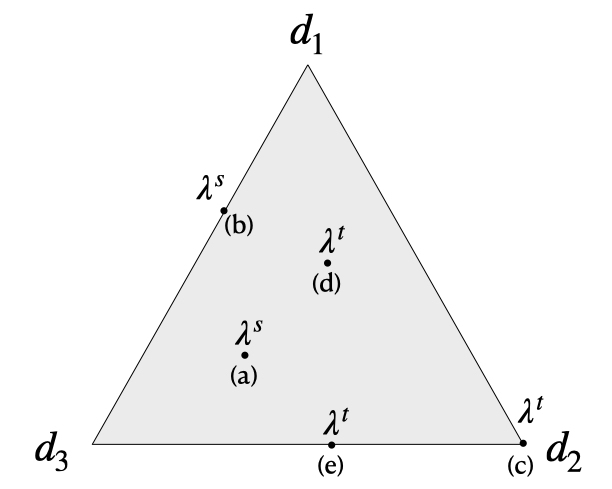
\includegraphics[width=0.5\textwidth]{graphics/mdmt-lambdas}
  \caption[Training and testing with distribution mismatch]{Training and testing with distribution mismatch. We consider just three domains, and represent vectors of mixture weights $\vlambda^{s}$ and $\vlambda^{t}$ in the 3-dimensional simplex. Training with weights in (a) and testing with weights in (c) is supervised multi-source domain adaptation to domain~2 ($d_2$), while (b)-(c) is the unsupervised version, with no training data from $d_2$; training with weights in (a) and testing with weights in (d) is multi-domain learning, also illustrated with configurations (a)-(e) (training domain $d_1$ is not seen in test), and (b)-(d)  (test domain $d_2$ is unseen in training).}
  \label{fig:mdmt-lambdas}
\end{figure}

This framework modelizes the real context closely because, in a typical setting in machine translation, we collect the most extensive collection of parallel data for the chosen language pair to achieve optimal performance for the task of interest. In such situations, the training data distribution is opportunistic. The test data distribution is determined and fixed; a key component in training is to mitigate the detrimental effects of a possible mismatch between these distributions. Training data may be a mixture of many domains such as the JRC-Acquis Communautaire corpus (\domain{law}-domain) \citep{Steinberger06acquis} or documentation for KDE, Ubuntu, GNOME and PHP from the Opus collection \citep{Tiedemann09news} (\domain{it}-domain). We also leverage a collection of data with no specific topic and genre, such as Paracrawl \citep{Banon20Paracrawl}. The testing data represent the domains of interest. In multi-domain adaptation, because there are multiple target domains, the testing is composed of multiple tests. The performance of an MT system is usually the average of its performance on these tests. However, we can access the quality of the multi-domain MT system with different priorities over target domains using weighted mean. The evaluation of multi-domain MT system should be clarified before training as early stopping criteria relies on the evaluation over validation tests.
\subsection{4 main sub-problems}
From our study on many previous works, we realize that the (multi-)domain adaptation problem is a multifaceted problem. Effectively, all the cases of (Multi-)domain adaptation can be classified into four groups by answering two following questions:
\begin{itemize}
	\item Is/Are the domain(s) of the training deterministic?
	\item Is/Are the domain(s) of the testing deterministic?
\end{itemize}
More precisely, the first question asks whether the training data is composed of a number of known domains. For example, the domain of a mixture of multiple corpora of specific topics, such as JRC-Acquis Communautaire corpus (\domain{law}-domain) and KDE (\domain{it}-domain), is well defined. However, the domains in Paracrawl \citep{Banon20Paracrawl} is unknown because it was built by crawling the content of web-sites without specifying topic or purpose. The second question asks whether the domain of the testing data is determined. If there exists a collection of text (monolingual or parallel) that defines the domain of the testing, then it is domain-deterministic and vice versa. 

Our first case of (multi-)domain adaptation \ref{sec:case1} is supervised multi-domain adaptation in which domain labels are both available in training and testing. Furthermore, the target domains in testing are included in the training. This case might be the most straightforward situation. Many approaches in multi-domain MT conducted their experiments in this setting \cite{Pham21revisiting}. 

The second case \ref{sec:case2} considers the use of the parallel data crudely collected from webs such as Paracrawl \citep{Banon20Paracrawl} or Commoncrawl \footnote{\url{https://commoncrawl.org/}}. The content of these corpora varies from many topics, but unfortunately, there is not any available domain label for sentences. Fortunately, in the second case, the target domains are known, i.e., there exist data of these domains, which can be used to adapt the model. The second case focuses on the exploitation of opportunistic text. 

The third case \ref{sec:case3} assumes a well domain-labeled training data while allowing the testing sentence from any possible domain. This case focuses on the robustness of the MT system against any possible shift distribution in testing. The third setting is very closed to real applications where the provenance of the input text is unknown. 

Finally, the last setting \ref{sec:case4} focuses on both exploiting opportunistic data in training and being robust against unknown testing distribution. We dedicate the four following sections to discuss more details of each setting.

Recently the work of \citet{Chu18survey} significantly captured the landscape of MT domain adaptation by categorizing previous methods in 2 main classes: data-centric and model-centric. The data-centric category includes methods that manipulate the training distribution to resemble the distribution of the target domain better. The model-centric methods focus on changing the architecture, modifying the training objective, and improving the inference.

According to \citet{Chu18asurvey}, the data-centric focuses on two paradigms, including 1) collecting parallel data related to the domain target, 2) creating synthetic data resembling the domain target. The first paradigm searches for similar examples to the ones of the domain target to enlarge the domain target's training data. The second paradigm aims to create pseudo examples resembling the data of the domain target. Besides the two paradigms, we propose another paradigm, which is data sampling. The data sampling paradigm consists of changing the data sampling distribution during the training course to mitigate the heterogeneity of the data size between domains and the variety of the "difficulty" of the domains. Therefore data-centric consists of 3 paradigms, including 1) data collection, 2) data synthesization, and 3) data sampling.

This taxonomy is largely adopted in MT domain adaptation's research. However, we find a naivety in this classification as it misses delivering an answer for the most ultimate question: "which method solves which problem?". We propose adding another dimension, the context of the MT adaptation problem, to form a Cartesian map of the MT (multi-)domain adaptation area. The four following sections will explain how model-centric and data-centric categories solve 4 (multi-)domain adaptation cases. We believe that this coupling of methods and cases will allow us to navigate better the (multi-)domain adaptation forest that has been growing for almost two decades. We also introduce several unexplored adaptation problems that need more research effort and other applications of existing application methods. The work of \citet{Pham21revisiting} recently gave a brief review of several well-known adaptation methods via a reevaluation with different domain adaptation cases. However, the experiments are still limited in the first case \ref{sec:case1} and the third case \ref{sec:case3} by excluding crawled corpora.

\section{Supervised (multi-)domain adaptation}
\label{sec:case1}
In the supervised (multi-)domain adaptation, the domain label is available in both training and testing. Furthermore, the domain(s) in testing is(are) available in training. In this problem, we would like to achieve a unique model that performs the best in one or many target domains, given training data from those domains and probably from other domains. This setting is the most popular situation on which multi-domain machine translation research papers focus. The first case represents the least requirement as the MT needs to achieve the best performance on the domains it learned from. The difficulty of this situation is to both exploit the proximity between domains while mitigating the interference due to inter-domain heterogeneity. Effectively, similar topics, such as legal and administrative, might improve the vocabulary coverage of each other as both domains share the same specific terminologies. However, distant topics, such as religion and IT might confuse the MT system when sharing the same parameters. In the following sections, we will discover how model-centric methods and data-centric methods solve this case.
\subsection{Model-centric}
In the case of the supervised multi-domain adaptation, model-centric methods focus on adding domain-specified parameters to reduce the interference between domains while keeping the number of parameters small. The simplest methods use domain tags. For example, \citet{Kobus17domain} proposed appending a special token to each source sequence indicating its domain such as $<Domain=IT>$ and train the NMT model with this format. However, this format requires domain tags in testing; hence we have to predict them if the source sentences are from an unknown origin. \cite{Britz17effective} originally proposed appending domain tag to the target sequence so that the decoder will predict the domain in which it will generate the translation. Instead of using domain tag, \citep{Kobus17domain, Pham19generic} proposed using domain embedding to incorporate the domain information into the context of the translation. \citet{Kobus17domain} concatenated an embedding of small size (e.g., 4) to the embedding of each token in the input sequence. Each small embedding corresponds to a domain. Instead of using the same domain embedding for the tokens in the same domain \citet{Pham19generic} used lexicalized domain representation, which is a small embedding correspond to the domain and the token. Besides domain embedding, we can use domain-specified layers that can be plugged between 2 consecutive layers of the NMT model without changing the architecture. There are 2 types of plug-in layers: 1) residual adapter \citep{Bapna19simple, Pham20Study} and 2) learning hidden unit contribution \citep{Vilar18learning}. Residual adapters were first introduced by \citet{Rebuffi17learning} in computer vision. \citet{Bapna19simple} proposed this fine-tuning paradigm for domain adaptation. They introduced a new version of residual adapter composed of 2 linear projections and the ReLU activation function. The adapters are plugged into the NMT model as follow
\begin{equation}
\begin{array}{rcl}
h_{enc/dec}^l = h_{enc/dec}^{l} + ADAP_{enc/dec}^l(h_{enc/dec}^{l})
\end{array}
\end{equation}
where $ADAP_{enc/dec}^l$ is the adapter corresponding to the $l^{th}$ layer of the encoder/the decoder. \cite{Pham20Study} studied the use of the residual adapters for multi-domain adaptation and propose several techniques, including regularization, gating mechanism, to improve the robustness of the model. The learning hidden unit contribution (LHUC \nomenclature[lhuc]{LHUC}{Learning hidden unit contribution}) method was proposed by \cite{Vilar18learning} to adapt an NMT model to a domain. The author applied an LHUC layer to the model as follow
\begin{equation}
h_{enc/dec}^l = h_{enc/dec}^{l} \odot a(\rho^{l}_{enc/dec})
\end{equation}
where $\rho^{l}_{enc/dec}$ is the adapter corresponding to the $l^{th}$ layer of the encoder/the decoder and $\rho^{l}_{enc/dec} \in \mathbb{R}^d$. $a(.)$ is a scaled
element-wise sigmoid function.
$$a(x) = \frac{2}{1+e^{-x}}$$
Residual adapter and learning hidden unit contribution layer adapt a pretrained model without changing its parameters. 

While the previous methods aim to discriminate domains to reduce the interference,\cite{Britz17effective} was motivated to learn hidden representations that are invariant between domains. More precisely, the authors use a binary classifier that takes the output of the encoder as input to distinguish the source sequences of 2 source domains. They inverse the sign of the gradient corresponding to the loss of the classifier to confuse it, i.e., making the hidden representation of the encoder invariant between 2 domains. This technique is related to A-distance, which is a measure of similarity between two probability distributions. \cite{Ben07analysis} showed that the A-distance between the
source and target distributions is a crucial part of an upper generalization bound for domain adaptation. They hypothesized that it should be difficult to discriminate between the source and target domains to have a good transfer between them because
this would imply similar feature distributions. \cite{Zeng18multidomain}'s work was also inspired by this idea. However, instead of forcing the encoder's output to be invariant between domains, the authors focus on extracting domain-agnostic features and domain-specific features from the output of the encoder and feeding the features to the decoder. To do that, they use two different non-linear transformations, which map a hidden representation to two vectors of the same size. Then, they apply one domain classifier on each extracted feature vector. The domain-agnostic feature vector is trained to confuse its corresponding classifier, whereas the domain-specific feature vector is trained to facilitate its classifier.

\cite{Michel18extreme} adapted a pretrained model to a multi-user personalized model by fine-tuning the
bias of the output softmax to each particular user of the MT system. The number of additional parameters is $|S| \times |\Sigma_y|$, in which $S$ is the set of the users. The author reduces the size of the bias matrix $B \in \mathbb{R}^{|S| \times |\Sigma_y|}$, whose each row is a bias vector of one user, by factoring it into lower dimension representation, i.e.
\begin{equation}
\begin{array}{rcl}
B &=& S \times \tilde{B}, \\
&where& \\
S & \in & \mathbb{R}^{|S| \times r}, \\
\tilde{B} & \in & \mathbb{R}^{r \times |\Sigma_y|}.
\end{array}
\end{equation}

\citet{Jiang20Multi}'s work was inspired by the mixture of expert paradigm. Their novel model is based on Transformer architecture \citep{Vaswani17attention} as they integrate a domain-mixing mechanism to the multi-head attention layer. As we explained in Section ~\ref{ssec:transformer-enc}, each head of multi-head attention layer is computed as follow
\begin{equation}
head_i = Attention \big(QW_i^Q, VW_i^V, KW_i^K \big).
\end{equation}
Suppose that there are $K$ domains, at the $i^th$ head, for each query, key and value component, there are $K$ transformation matrix $W_{i,j}^Q | j \in [1,K]$, $W_{i,j}^K | j \in [1,K]$, $W_{i,j}^V | j \in [1,K]$ respectively. The domain-mixing mechanism is applied on query, key and value components as follow
\begin{equation}
\begin{array}{rcl}
Q_i^t &=& \sum_{j=1}^K Q^tW_{i,j}^Q*\mathit{D}_j(x_t),\\
K_i^t &=& \sum_{j=1}^K K^tW_{i,j}^K*\mathit{D}_j(x_t),\\
V_i^t &=& \sum_{j=1}^K V^tW_{i,j}^V*\mathit{D}_j(x_t),\\
head_i &=& Attention \big( Q_i, K_i, V_i\big),
\end{array}
\end{equation}
where the subscript $t$ indicates the position of the vector in the sequence of hidden representations, $\mathit{D}(x_t) \in \mathbb{R}^{K}$ is the domain proportion of the corresponding token $x_t$. The proportion of domains of a token is computed by a domain classifier, that take the input embedding of that token as input. The novel model adapt the hidden representation of a token to a domain to which the token likely belongs. Therefore, the model is able to discriminate domains in domain-specific tokens while transfering knowledge between domains in domain-agnostic tokens. However, the size of the model is proportional to the number of domains, which is not practical in the real applications. However, in our opinion, the idea can be applied to lightweight adapter or learning hidden unit contribution layer.

Besides the model-centric methods related to the architecture, multi-task training is another solution to the supervised (multi-)domain adaptation problem. 

We illustrate several well-known model-centric methods for the supervised domain adaptation problem in Figure~\ref{fig:model-centric-case1-case2}.
\begin{figure}[htbp]
\begin{subfigure}{1.0\textwidth}
  \centering
  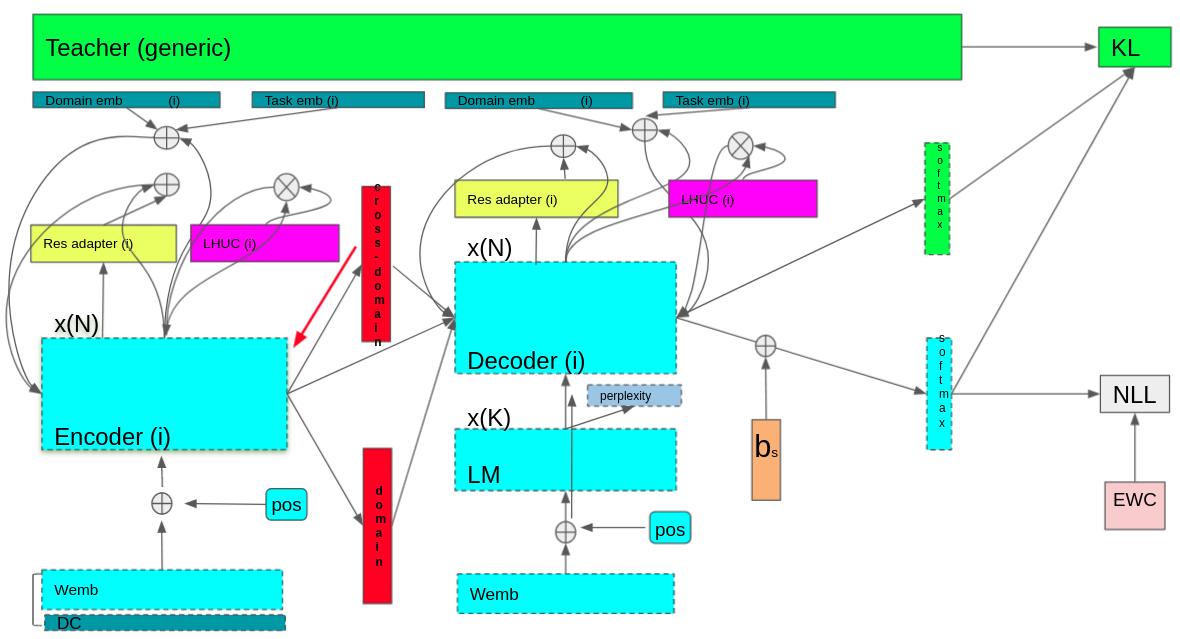
\includegraphics[width=1.0\textwidth]{graphics/supervised_mdmt}
\end{subfigure}
\newline
\begin{subfigure}{1.0\textwidth}
  \centering
  \fbox{\begin{tabular}{ll}
\textcolor{red}{$\blacksquare$} & \citep{Zeng18multidomain} \\
\textcolor{violet}{$\blacksquare$} & \citep{Vilar18learning} \\
\end{tabular}}
\end{subfigure}
\caption[Model-centric's brief overview]{Each color different from the bleu corresponds to one model-centric method. The bleu represents the NMT model.}
\label{fig:model-centric-case1-case2}
\end{figure}

\subsection{Data-centric}
\subsubsection{Data sampling}
In supervised multi-domain adaptation, data sampling approaches aim to balance the contribution of each domain to the final model. In an opportunistic multi-domain training data, the data size of each domain vary from few thousands examples to millions examples. In a trivial mixture of data, small domains are usually excessively under-sampled causing a sub-optimal performance in average. However, if we equally sample data from every domain, the NMT model is easily over-fitted in the small domains. Therefore, finding optimal sampling distribution of domains is essential. \cite{Wang20balancing} proposed parameterizing the probability of sampling data from a domain and learned this probability via REINFORCE algorithm \citet{Williams92simple} using rewards computed from cosine-similarity between the gradient over in-domain training data and the gradient over dev-sets' data. We compare this technique to our approach in chapter \fyTodo{add reference of chapter MDAC here}.

Other data-centric methods, that does not take into account the domains of the training data will be discussed in Section ~\ref{ssec:case-2-data}.
\section{Non domain-deterministic training, domain-deterministic testing}
\label{sec:case2}
In this situation, the training data is composed by a number of unknown domains. The second case focuses on adapting the NMT model with an unknown source domain while the target domain is well defined. There are two situations: 1) there exists parallel data in the target domain 2) there exists only monolingual data in the target domain. The two following sections will discuss how each group of method solve these cases.
\subsection{Model-centric}
First, we discuss the case with one target domain in which there exist parallel data. In this case, we can apply the same techniques proposed for supervised (multi-)domain adaptation by considering the source domain as a generic domain. Besides, fine-tuning is very efficient approach for this problem\citep{Luong15stanford,Miceli17regularization,Servan16Domain,Freitag16fast}. We first train an NMT model with the mixture of source domains, then continue training this model with the parallel data of the target domain. According to a recent review of multi-domain adaptation conducted by \citet{Pham20Priming}, fine-tuning is the strongest baseline in supervised domain adaptation. However, fine-tuned NMT models usually suffer from catastrophic forgetting \citep{Michael89catastrophic} as their performances drop dramatically in the source domains. To mitigate the catastrophic forgetting, several regularization techniques were introduced, including mixed fine-tuning \citep{Chu17empirical}, uniform weight-decay \citep{Miceli17regularization}, elastic weight consolidation (EWC \nomenclature[ewc]{EWC}{Elastic weight consolidation}) \citep{Brian19overcoming, Kirk16overcoming, Saunders19domain} and knowledge distillation \citep{Dakwle17fine}. 

Mixed fine-tuning \citep{Chu17empirical} adapts an NMT model with the mixture of the source domain and the target domain (by oversampling the target domain). The method adapts the NMT model to the domain of interest thanks to the oversampling while maintaining its robustness to generic text as it is trained with the source domain.

Weight decay \citep{Miceli17regularization} continues the training on the target domain's data with a regularized loss 
\begin{equation}
L_{CE}(\theta,\mathit{D}_{target}) + \alpha * \parallel \theta - \theta^{A} \parallel_{L_2},
\end{equation}
where $\theta^{A}$ is the value of the pretrained model. Fine-tuning with the new loss fits the model to the target domain while preserving the parameters' old pretrained values, therefore preventing the overfitting of the NMT model in the target domain and maintaining the generality over source domains. \citet{Brian19overcoming, Kirk16overcoming, Saunders19domain} were also motivated to penalize the changes of the parameters compared to the old model. However, the authors argued that not every parameter has the same contribution to maintain the generality to the old domains and that we can tune the parameters unimportant to the old domains to the target domain. The contribution of each parameter of the pretrained model is approximated by the diagonal of the Fisher matrix computed over the data of the source domains. Therefore, fine-tuning with EWC uses the following loss
\begin{equation}
L_{CE}(\theta,\mathit{D}_{target}) + \sum_{i} \frac{\lambda}{2} F_i * (\theta_i - \theta_i^{A})^2,
\end{equation}
where the $F_i$ is the $i^th$ element of the diagonal of the Fischer matrix approximated as follow
\begin{equation}
\bar{F} = \frac{1}{|\mathit{D}_{source}|} \displaystyle{\mathop{\sum}_{(x,y)\in \mathit{D}_{source}}} \nabla log(p(y|x,\theta))_{| \theta^{A}} \nabla log(p(y|x,\theta))_{| \theta^{A}}^{T}
\end{equation}
\citet{Dakwle17fine}'s method was motivated by knowledge distillation paradigm \citep{Hinton15Distilling}. The authors propose regularizing the standard cross-entropy loss with the Kullback-Leibner distance \citep{Kullback51On} between two predicting distributions produced by old model and new model as follow
\begin{equation}
L_{CE}(\theta,\mathit{D}_{target}) + \alpha * \displaystyle{\mathop{\sum}_{(x,y)\in \mathit{D}_{source}}} KL(p(.|x,\theta) | p(.|x,\theta_{A})).
\end{equation}

Instead of continuing the training with target domain only, \citet{Chen17cost} differentiated directly domain-relevant instances and irrelevant instances via instance weighting. The authors compute the weight of each instance by a domain classifier, that is trained with source sequences. The training will maximize the following objective 
\begin{equation}
\begin{array}{rcl}
\hat{\theta} = \displaystyle{\mathop{\arg max}_{\theta} \mathop{\sum}_{(x,y)\in D_{in} \cap D_{out}}} (1+p_d(x))log(P(y|x,\theta))
\end{array}
\end{equation}
where $D_{in}$, $D_{out}$ are the target domain and other domains, $p_d(x)$ is the probability that $x$ comes from the target domain. \citet{Wang17instance} proposed using different domain-relevance metric for instance weighting. 

Besides the auxiliary losses, ensemble methods are also promising. For example, \citet{Freitag16fast} proposed ensembling the pretrained model and the fine-tuned model to combine the advantage of both models: the specialization in the target domain and the generalization over general text.

Still in the case of the uni-domain adaptation, but without parallel data. The model-centric approaches mostly use monolingual data in the target language of the target domain. The proposed methods mostly adapted the decoder to the target domain. For example, \citet{Gulcehre16monolingual} proposed training a language model adapted to the target domain and fusing the language model to the decoder. The fusion could be deep or shallow. The deep fusion combined the hidden representation of the decoder and the one of the language model before computing the prediction probability. The shallow fusion combined the prediction probability computed by the decoder and the one computed by the language model. \citet{Domhan17using} was also motivated by this idea. However, the authors proposed jointly training the language model and the NMT model via multi-task training. Furthermore, the decoder and the language model shared the word embedding of the target side.

All previous methods were motivated to adapt an NMT model to a specific domain. We realize that they can hardly be applied to multi-domain adaptation because all the parameters of the MT model are adapted to one domain. However, in the case where there are parallel data of the target domains, we could use model-centric methods proposed in the supervised adaptation by considering the training domain a generic domain. Recently, \cite{Dou19unsupervised} proposed using domain-embedding and task-embedding to adapt an NMT model to the target domain using reconstruction loss on the monolingual data. More precisely, for each layer $l^{th}$ of an ANMT model, there are 2 task embeddings $\theta_{task}^{\gamma,l}$, $\gamma \in \{ MT, LM \}$, which correspond to translation task and language modeling task respectively. Furthermore, for each layer $l^{th}$, and for each domain $d$, there is a domain task $\theta^{d,l}_{dom}$. The layer $l^{th}$ of encoder/decoder will be as follow
\begin{equation}
h^{l} = LAYER^l(h^{l_1}) + \theta^{d,l}_{domain} + \theta_{task}^{\gamma,l}
\end{equation}
Now, the parallel data will be used to compute translation loss, while the monolingual data is used to compute language modeling loss. The authors proposed adding noises to the source sequence while computing the LM loss. Using domain-specific embeddings enables the model to be adapted to multiple domains at once. Despite being applied to multi-lingual machine translation, the monolingual adapter proposed by \citet{Philip20monolingual} shares the same spirit and can be applied to this situation.
\subsection{Data-centric}
\label{ssec:case-2-data}
According to our study, the previous data-centric approaches proposed to this situation belong to all three paradigms, including data selection, data synthesization, and data sampling. The two following sections will discuss the methods of each paradigm.
\subsubsection{Data selection}
Data selection approaches collect parallel data, which resemble the target domain. The selection is usually based on a score of proximity between a parallel example and the domain. The score of proximity can be computed via sentence embedding or variants of \citeauthor{Moore10intelligent} score. For example, given two corpora of a target domain $D_{I-src}$, $D_{I-tgt}$ and two corpora of the source domain $D_{O-src}$, $D_{0-tgt}$, \cite{Axelrod11domain} computed a bilingual version of Moore $\&$ Lewis score of a sentence pair as follow
\begin{equation}
\begin{array}{rcl}
S_{bi} (x,y) &=& H_{I-src}(x) - H_{O-src}(x) + H_{I-tgt}(y) - H_{O-tgt}(y), \\
\end{array}
\label{eq:ced}
\end{equation}
where the cross-entropy $H_{*}(z)_{| * \in [I-src, I-tgt, O-src, O-tgt], z \in [x,y]}$ of the sentence $z$ is computed by a language model trained only with the corpus $D_{*}$. \citet{Duh13adaptation} proposed the same formulation as proposed \citet{Axelrod11domain} but used a neural language model instead of a statistic language model. In a survey of data selection methods for neural machine translation, \citet{Silva18extracting} evaluated 3 popular methods in the domain adaptation task, including cross-entropy difference, Term Frequency-Inverse Document Frequency (TF-IDF \nomenclature[tf-idf]{TF-IDF}{Term Frequency-Inverse Document Frequency}) \citep{Salton73On} and Feature Decay Algorithm (FDA) \citep{Poncelas18Feature}. More precisely, cross-entropy difference was performed as described above and normalized by sentence length. To perform TF-IDF, \citet{Silva18extracting} consider each sentence of the target domain as a query and every sentence in the source domain as a key. The tf-idf vectors of the queries and the keys are computed as in \citet{Salton73On}. The score of proximity between a query and a key is the cosine-similarity of theirs tf-idf vectors. Based on the score of proximity, for each sentence of the target domain, we retrieve K nearest-neighbors in the source domain. The collection of the retrieved sentences is the result of the method. The last method FDA extracts from the source domain a set of sentences that better represent a given test set provided by the source side of the target domain. \revision{The detail of the algorithm is referred to the work of \citet{Poncelas18Feature}.}

\cite{Wang17sentence} proposed using sentence embedding to represent a sentence instead of a tf-idf vector. For each language side (source/target) the authors computed the centroid of the target domain and one of the source domain. Assume $C_{E_{in}}$, $C_{E_{out}}$ are the centroid of the target domain and the source domain in the source language,  $C_{F_{in}}$, $C_{F_{out}}$ are the centroid of the target domain and the source domain in the source language, $v_{\mathit{e}}$ is the sentence embedding of a source sentence $\mathit{e}$, $v_{\mathit{f}}$ is the sentence embedding of a source sentence $\mathit{f}$, then the proximity of the example $(\mathit{e},\mathit{f})$ to the target domains is defined as follow
\begin{equation}
d(v_{\mathit{e}}, C_{E_{in}}) - d(v_{\mathit{e}}, C_{E_{out}}) + d(v_{\mathit{f}}, C_{F_{in}}) - d(v_{\mathit{f}}, C_{F_{out}}),
\end{equation} 
where $d(.,.)$ is the Euclidean distance in $\mathbb{R}^d$. \cite{Aharoni20unsupervised} proposed using sentence embedding computed by a pretrained Bidirectional Encoding Representation Transformer (BERT \nomenclature[bert]{BERT}{Bidirectional Encoding Representation Transformer}) and the cosine-similarity to retrieve domain-related examples.

\subsubsection{Data synthesization}
The most efficient approach of this paradigm is backtranslation \citep{Sennrich16improving}, which consists of translating the monolingual data of the target language to the source language. \citet{Burlot18using} showed significant improvement of an NMT model in the target domain when trained with the mixture of parallel data and the in-domain backtranslated data. Without backtranslating the target-side data, \citet{Currey17copied} created artificial sentence pairs from the monolingual data in the target language so that each source sentence is identical to the target sentence. Training an NMT model with the mixture of parallel data and artificial sentences improves the accuracy of the translation on named entities and other words that should remain identical between the source and target languages. 

\subsubsection{Data sampling}
Data sampling methods dynamically change the composition of the training data over time. A difference between data sampling and data selection is that data sampling does not keep the same training data after the collection. However, the two paradigms are orthogonal. In practice, the evolution of the training data is beneficial for training an NMT model specialized to a domain. For example, fine-tuning is similar to this paradigm as the training begins with every available data and finishes with the data of the target domain. However, data sampling methods consist of building an automatic curriculum without human supervision. For example, \citet{Wees17dynamic} proposed gradual fine-tuning, which first computes a sampling distribution based on the cross-entropy difference (CED) \eqref{eq:ced} of each example, then gradually decreases the number of examples sampled from previous distribution for each epoch. Formally, the CED score of each example is normalized as follow
\begin{equation}
\tilde{CED}(x) = 1 - \frac{CED(x)-min(CED_{G})}{max(CED_{G}) - min(CED_{G})},
\end{equation}
where $G$ is the training corpus. Therefore the higher-ranked example has a higher $\tilde{CED}$ score rather than having lower $CED$ as in \cite{Axelrod11domain}. The sampling distribution is computed as follow
\begin{equation}
\omega(x) = \frac{\tilde{CED}(x)}{\sum_{x'\in G} \tilde{CED}(x')}.
\end{equation}
For each epoch $i^{th}$, a number $n_i$ of examples are selected according to the previous distribution. $n_i$ is defined as follow
\begin{equation}
n_i = \alpha \cdot |G| \cdot \beta^{\lfloor \frac{i-1}{n}, \rfloor}
\end{equation}
where $\alpha \in [0,1]$ is the relative start size, $\beta \in [0,1]$ is the retention rate. Via the same mechanism, \citet{Wang19dynamically} proposed a more sophisticated dynamical sampling distributions combining two scores of an example, including domain-CED and noise-CED. The authors proposed two variants, including mixed co-curriculum, which score an example by the sum of its CED scores, and cascaded co-curriculum, which first selects examples by domain-CED then retains top examples according to noise-CED from previous selection. Furthermore, \citet{Wang19dynamically} proposed to recompute the language model of noisy data for each epoch. Instead of increasing the domain-relevance of the training data, \cite{Zhang19curriculum} did the opposite. More precisely, they reordered the training data according to their relevance to the target domain then equally split the whole corpus into many shards containing samples of a similar score. They trained an NMT model with one shard per epoch in decreasing order of domain-relevance.

Besides well-known metrics for domain-relevance, \citet{Zhang19curriculum} proposed a parameterized scorer, that evaluates the usefulness of each sample to the performance on the target domain, and optimized its parameters via Bayesian optimization. More precisely, the scorer was formulated as follow
\begin{equation}
\mathit{f}(x,y) = V \cdot \mathbf{F}(x,y),
\end{equation}
where feature vector $\mathbf{F}(x,y)$ was extracted from the example, and weight vector $V$ was learned by Bayesian optimization. Each element of $\mathbf{F}(x,y)$ represented the relevance of the example to a target domain. Once the scorer was optimized, the training was conducted similarly as in \citet{Wees17dynamic,Wang19dynamically}.

\section{Domain-deterministic training, non domain-deterministic testing}
\label{sec:case3}
The third case is interesting because it resembles the real context of machine translation's applications. Effectively, the users' text can be from any possible topic or for any possible purpose (genre). In this situation, the NMT model needs to be both robust to the unseen domains and adapted to the known domains. 
\subsection{Model-centric}
Mixture model is effective to this situation as it combines domain-adapted systems to perform the translation. Effectively, the performance of mixture model is guaranteed in the source domains while using a convex combination of the adapted systems is robust against the unseen domains. Mixture model has been successfully applied for SMT models \citep{Sennrich12perplexity, Carpuat14linear, Sennrich12mixture}. \citet{Sajjad17neural, Saunders19domain,Freitag16fast} applied mixture model to NMT models. The contribution of each adapted model to the combination was uniform in \citet{Freitag16fast} while \cite{Sajjad17neural} pre-finetuned them by bayesian optimization on a development set. However, heuristic static weight is sub-optimal when the testing domain is highly variable. \citet{Saunders19domain} proposed computing the weights of the mixture for each source sentence $x$ at $i^{th}$ decoding step as follow
\begin{equation}
\begin{array}{rcl}
W_{k,i} &=& \displaystyle{\mathop{\sum}_{t} P(t|h_i,x)\lambda_{k,t}}, \\
&where& \\
P(t|h_i,x) = P(t|x) &=& \frac{\displaystyle{P^k_{LM}(x)}}{\displaystyle{\mathop{\sum}_{k'} P^{k'}_{LM}(x)}},\\
\end{array}
\end{equation}
where $P^{k'}_{LM}(x)$ is the probability of the source sentence $x$ according to the language model learned from domain $k'$, $\lambda_{k,t}$ can be uniform, identity or pre-finetuned with a development set. \citet{Saunders19domain} also proposed varying the mixture's weights during the inference by conditioning the domain posterior probability on both $x$ and $h_i$ as follow
\begin{equation}
P(t|h_i,x) = \frac{P(h_i|t,x) P(t|x)}{\displaystyle{\mathop{\sum}_{k'} P(h_i|k',x) P(k'|x)}}.
\end{equation} 
However, one might be more interested in domain robustness than domain specialization. The mixture model does not include the domain robustness in the training objective. \cite{Muller20domain} discussed several regularization methods to mitigate the problem, including subword regularization \citep{Taku18subword}, defensive distillation \citep{Papernot16distillation}, reconstruction \cite{Tu17neural} and neural noisy channel reranking \citep{Li16mutual}. Distributional robustness \citep{Oren19distributionally,BenTal13robust} is also a promising paradigm as the methods optimized learning models so that they perform well over a wide range of potential test distributions. However, the application of this paradigm to neural machine translation is not yet discovered.
\subsection{Data-centric} \label{ssec:data-centric}
Data-centric can not be applied to this situation as non domain-deterministic testing does not provide the domain of the test sentences. Effectively, data-centric requires the monolingual data of the target domain to create the pseudo in-domain data while the testing domain is non deterministic.
\section{Non domain-deterministic training, non domain-deterministic testing}
\label{sec:case4}
\subsection{Model-centric}
\cite{Li18onesentence, Farajian17multidomain} proposed finetuning on-the-fly the pretrained model to a mini-batch similar to the source sentence before translating it. The authors chose the learning rate and the number of finetuning iterations according to the score of similarity between the mini-batch and the source sentence so that the higher similarity the higher the learning rate, the more iterations. \cite{Pham20Priming,xu20boosting,Bulte19neural} proposed learning NMT model to reuse memory translations whose source sentence is similar to the source sentence. 
\subsection{Data-centric}
The data-centric paradigm can not be applied to this situation for the same reason as the previous section \ref{ssec:data-centric}














































































































































































































































































































































































